\subsection{Motivation}
% One of the goals of phonology is to develop predictive models of phonotactics.
% Such models predict phonotactic judgments of words based on various properties
% of those words, UG, and the language's lexicon. In order to enable us to choose
% more effective models, I propose to investigate the correlation between the
% number of phonotactic violations in a word and the phonotactic judgment it
% elicits.

In modeling constraint-based phonotactics, there are three broad kinds of decisions to be made: which framework
to use, which parameters (constraints) to use, and how to tune (rank or weight) the parameters. This experiment
aims to offer support for a particular framework, freeing up phonologists to focus on the latter decisions.

Popular constraint-based frameworks include Optimality Theory \citep{Prince1993/2004}, Harmonic Grammar (taken here to mean linear Harmonic
Grammar, in which harmony scores are not subject to exponentiation) \citep{Legendre1990c,Smolensky2006b,Pater2009,Potts2010}, and Maximum Entropy
\citep{Goldwater2003}.



%Ohala and Ohala 1986

% It may be linear, so that each additional violation of equal
% magnitude decreases judgments equally, or it may be nonlinear, so that
% additional violations have increasing or decreasing contributions to judgments.

Optimality Theory predicts that adding mild
violations to a word with a severe violation has no effect, so that the
function from number of violations to grammaticality is flat for any given
first violation as long as it remains one of the worst violations in the word.

However, predating OT, \citet{Ohala1986} found that speakers have an above
chance probability of preferring a word with one violation to a word with that
same violation and a less severe one, suggesting that even the milder violations
affect the grammaticality of a word. Additionally, \citet{Coleman1997} found
that a word like \textit{mrupation}, with one severe violation followed by a
common English sequence, was preferred to a word like \textit{spleitisak}, with
several minor violations.  \citet{Albright_clusters_2008} designed experiments
to directly test the question of cumulativity of violations, addressing
potential alternative explanations for these two results, and found that models
that take into account all violations of a word, not just its worst violation,
fit the data significantly better.

%Sorace and Keller 2004 found cumulativity of violations for syntax
%TODO discuss grammaticality vs acceptability vs ratings

However, Albright did not compare various cumulative models against each other.
The shape of the curve relating number of violations to phonotactic judgments
bears on the question of which framework we should use to model phonotactic
well-formedness. As \citet{Pater_cumulative_2008} points out, Harmonic Grammar
predicts a well-restricted set of cumulativity effects, unlike Optimality
Theory with Local Constraint Conjunction \citep{Smolensky2006d}.
But the weighted constraints of Harmonic Grammar can be combined in a linear fashion,
producing the framework commonly associated with the name, or exponentiated and normalized,
as in Maximum Entropy. These approaches predict differently shaped curves.

\ex. Harmonic Grammar: The harmony $\mathcal{H}$ of a word $x$ is the dot product of the violation vector $v$,
representing violations of $x$ on each constraint in the constraint set $C$, with the constraint
weight vector $w$.\\
\[\mathcal{H}(x) = \sum_{i \in C}{v_iw_i}\]

\ex. Maximum Entropy: The probability $p$ of a word $x$ is the exponentiated negative harmony
of the word, normalized relative to the candidate set $X$.\\
\[p(x_i) = \frac{\exp(-\mathcal{H}(x_i))}{\sum_{j \in X}{\exp(-\mathcal{H}(x_j))}}\]

Consider a constraint with a weight
of two and candidates A, B, C, and D that violate it zero, one, two, and three
times respectively. In linear Harmonic Grammar, the candidates have the harmony scores
0, -2, -4, and -6; they decrease by two each time, in a linear pattern. In
Maximum Entropy, if we assume these candidates exhaust the possibilities, they
have the probabilities 0.865, 0.117, 0.015, and 0.002; candidate A has the
majority of the probability because it is the best choice available, and each
additional violation decreases the probability by a smaller amount than the
last.

\ex. 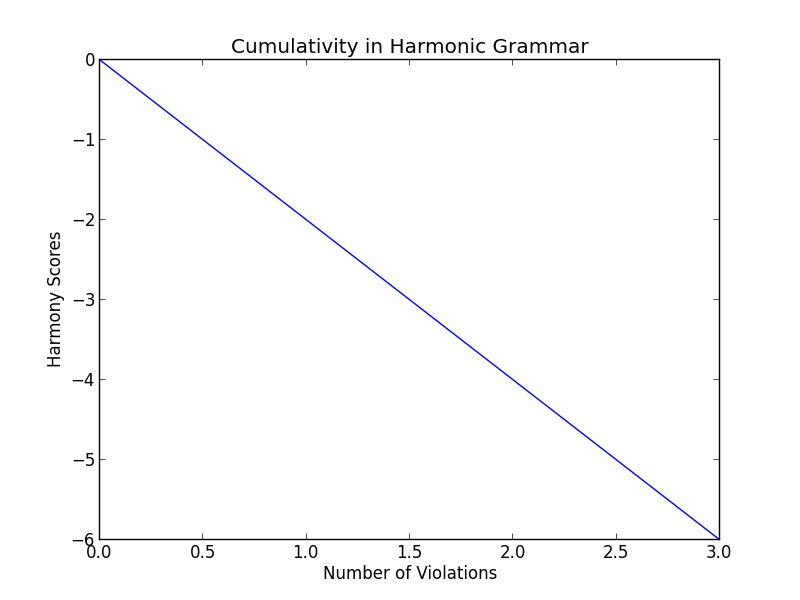
\includegraphics[scale=.5]{hg_cumulativity.png}

\ex. 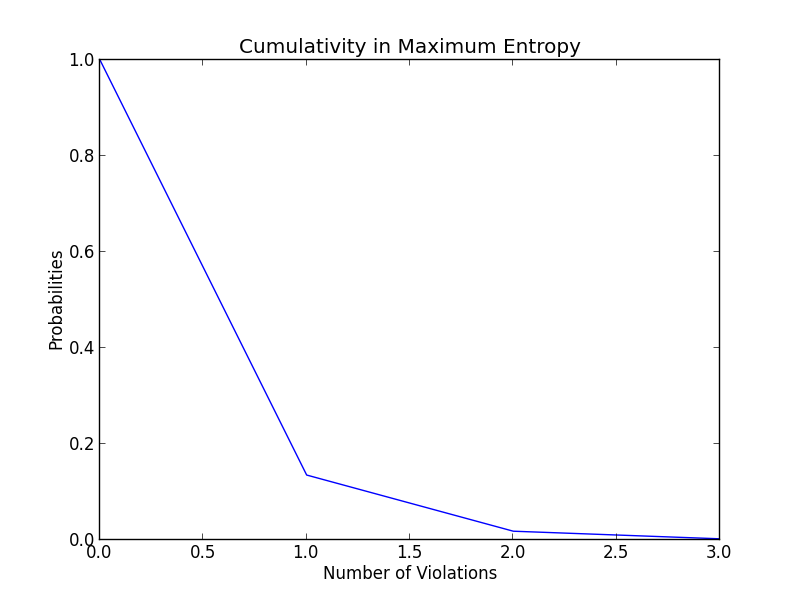
\includegraphics[scale=.5]{me_cumulativity.png}

I predict that, in accordance with the Maximum Entropy model, additional violations
will have smaller effects on the grammaticality of the word, as the grammaticality approaches a floor.


%In order to simplify this investigation, I will not attempt to define the set of patterns
%that can be considered phonotactic violations. Rather, I will use controlled experiments
%dealing only with patterns that are widely accepted to belong to that set for the language
%in question.

\subsection{Plan}

\citet{Albright_clusters_2008} has shown that cumulative models of phonotactics fit data
better than noncumulative ones. He used two types of words, those with
phonotactic violations in the onset and those with phonotactic violations in
the onset as well as milder violatinos in the rime. In a variety of analyses,
he fitted models that rate words by their worst violation only, and ones that
rate words by the sum of all their violations. The models that take into
account all violations in the word were more strongly correlated with experimental
findings. This study showed that cumulative models reflect speaker judgments better
than noncumulative models, but did not distinguish among various cumulative models.

I will ask which kind of cumulative model best fits the data.  Relative to
words with one violation, does the same violation add less, the same amount, or
more ungrammaticality to the word when it appears in a word that already has
another violation?

Each of 24 test items will appear in four conditions. The four conditions are created by
crossing two factors: presence of an onset violation and presence of a rime
violation.  Within an item, the onset violation will be the same whenever it is
present, and likewise for the rime violation. This way, comparing an item with
an onset violation only to the same item with both violations directly shows
the effect of the rime violation. The vowel is held constant across all conditions of an item.

Aside from test items, there will also be filler items. These will be nonce words
of medium acceptability; they will have mild violations that are different from the
kinds of violations found in the test words. Instead of violating cluster phonotactics,
they will violate long-distance OCP constraints or constraints on the cooccurrence of certain
vowels and codas. The goal is to keep participants from comparing filler and test items
piecewise and encourage them to use the filler only to get a sense of a baseline of grammaticality
against which to compare the test words. Fillers will be paired with sets of test items in a way
that minimizes overlap of OCP violating segments with test word segments.
%Participants will be asked to rate these words on a scale from one to four, as
%even-numbered scales allow for better detection of participants that are
%answering randomly.

Participants will be shown pairs of items and asked to choose the one that sounds
more like a possible word of English. Pairs will be composed of one of the test items
and one of the filler items. For each test item, each of its conditions will be compared
against the same set of filler items. A given participant will only see one of these pairings
for each item and filler word, thanks to a Latin Square design.

A mixed effects model will be fitted to the results. The dependent variable
will be proportion of times the test item was chosen. OnsetViolation,
RimeViolation, and their interaction will serve as fixed effects in addition
to random effects for subject and item. % separately for test item and filler item?

The purpose of the experiment is to test whether an interaction exists between
the two fixed effects. Bayesian methods will be used in the case of a null effect
to determine whether the absence of a significant interaction is likely to represent
a truly linear relationship as violations are added.

If a positive interaction is present, this would support a model that takes probability
away from words in greater and greater amounts as the number of violations increases.
I do not know of such a model, and this result is not predicted.

A negative interaction would support models like Maximum Entropy, in which each additional
violation subtracts less probability from the word than the last violation did.

A linear relationship would support models like linear Harmonic Grammar, in which each
additional violation subtracts the same amount of probability from a word as the last
violation did.


% another experiment: what do preference proportions (analogous to ratings) mean?
% - ratings on a scale are hard to interpret
% - proportions taken from 2afc tasks are better - more sensitive, more explicit
% - but still, what do they represent? how reliable are they?
% - do you pick A over B with a ratio of (ratio of A over C / ratio of B over C)?
% - if not, what does that mean?

